% ****** Start of file apssamp.tex ******
%
%   This file is part of the APS files in the REVTeX 4.2 distribution.
%   Version 4.2a of REVTeX, December 2014
%
%   Copyright (c) 2014 The American Physical Society.
%
%   See the REVTeX 4 README file for restrictions and more information.
%
% TeX'ing this file requires that you have AMS-LaTeX 2.0 installed
% as well as the rest of the prerequisites for REVTeX 4.2
%
% See the REVTeX 4 README file
% It also requires running BibTeX. The commands are as follows:
%
%  1)  latex apssamp.tex
%  2)  bibtex apssamp
%  3)  latex apssamp.tex
%  4)  latex apssamp.tex
%
\documentclass[superscriptaddress,unsortedaddress,
%runinaddress,
%frontmatterverbose, 
%preprint,
%preprintnumbers,
%nofootinbib,
%nobibnotes,
%bibnotes,
 amsmath,amssymb,
 aps,
%pra,
%prb,
%rmp,
%prstab,
%prstper,
%floatfix,
]{revtex4-2}

\usepackage{amsmath}
\usepackage{amsthm}
\usepackage{amssymb}
\usepackage[top=4cm,bottom=4cm,left=2.8cm,right=3.75cm,asymmetric,twoside]{geometry}
\usepackage{graphicx}
\usepackage{fancyhdr}
\usepackage{comment}
\usepackage{tikzorbital}
\usepackage{array} % center tables + 2 next lines
\newcolumntype{P}[1]{>{\centering\arraybackslash}p{#1}}
\newcolumntype{M}[1]{>{\centering\arraybackslash}m{#1}}
\usepackage{multirow} % confusion matrix
\newcommand\MyBox[2]{
  \fbox{\lower0.75cm
    \vbox to 2.0cm{\vfil
      \hbox to 2.0cm{\hfil\parbox{1.4cm}{#1\\#2}\hfil}
      \vfil}%
  }%
}
\usepackage{grffile}
\usepackage{epigraph} % quote
\usepackage{wrapfig} %wrapping text to fig
\usepackage{tikz} %draw figures

\usepackage{subcaption} %subcaption
\usepackage[font=small,labelfont=bf,width=0.9\textwidth]{caption}
\captionsetup[table]{skip=10pt}
\usepackage[T1]{fontenc}
\usepackage[sc, osf]{mathpazo}
\usepackage[euler-digits]{eulervm}
\usepackage{booktabs}
\usepackage{enumerate}
\usepackage{commath}
\usepackage{mathtools}
\usepackage[utf8]{inputenc}
\usepackage{pgfplots}
\usepgfplotslibrary{groupplots,dateplot}
\usetikzlibrary{patterns,shapes.arrows, arrows.meta,bending, shapes,calc,fadings,decorations.pathreplacing,positioning,arrows.meta}
\pgfplotsset{compat=newest}

\usepackage{sansmath}
\tikzset{>=stealth,
OptimumStyle/.style={align=center,anchor=east,rotate=90,font=\scriptsize}
}
\pgfplotsset{%samples=101,
axis lines = left,
every axis plot/.append style={line width=2pt},
}
% Include font for the identity operator
\usepackage{dsfont}
\usepackage[binary-units=true]{siunitx}
\usepackage{makecell}
\usepackage{longtable}
\usepackage{dcolumn}% Align table columns on decimal point
\usepackage{bm}% bold math
\usepackage{physics}
\usepackage{lipsum}
\usepackage{siunitx}
\usepackage{color}
\sisetup{separate-uncertainty}
\pgfplotsset{%samples=101,
axis lines = left,
every axis plot/.append style={line width=2pt},
}

\newcommand{\oliver}[1]{\textcolor{violet}{#1}} 
\newcommand{\morten}[1]{\textcolor{green}{#1}}
\newcommand{\sebastian}[1]{\textcolor{cyan}{#1}}
\newcommand{\marianne}[1]{\textcolor{blue}{#1}}
\newcommand{\oyvind}[1]{\textcolor{maroon}{#1}}
\newcommand{\lasse}[1]{\textcolor{red}{#1}}

\begin{document}

\title{Supplementary Material \\ 
%Predicting Solid State Qubit Candidates}
Predicting Solid State Material Platforms for Quantum Technologies}


\author{Oliver Lerst{\o}l Hebnes}
\affiliation{Department of Physics and Center for Computing in Science Education, University of Oslo, N-0316 Oslo, Norway}
\affiliation{Sopra Steria, N-0185 Oslo, Norway}

\author{Marianne Etzelm\"uller Bathen}
\affiliation{Advanced Power Semiconductor Laboratory, ETH Zürich, 8092  Zürich,  Switzerland}
\affiliation{Department of Physics and Center for Materials Science and Nanotechnology, University of Oslo, N-0316 Oslo, Norway}

\author{{\O}yvind Sigmundson Sch{\o}yen}
\affiliation{Department of Physics and Center for Computing in Science Education, University of Oslo, N-0316 Oslo, Norway}

\author{Sebastian G. Winther-Larsen}
\affiliation{Menon Economics, N-0369 Oslo, Norway}
\affiliation{Department of Physics and Center for Computing in Science Education, University of Oslo, N-0316 Oslo, Norway}

\author{Lasse Vines}
\affiliation{Department of Physics and Center for Materials Science and Nanotechnology, University of Oslo, N-0316 Oslo, Norway}

\author{Morten Hjorth-Jensen}
\affiliation{Department of Physics and Astronomy and Facility for Rare Ion Beams, Michigan State University, East Lansing, MI 48824, USA}
\affiliation{Department of Physics and Center for Computing in Science Education, University of Oslo, N-0316 Oslo, Norway}

\pacs{02.70.Ss, 31.15.A-, 31.15.bw, 71.15.-m, 73.21.La}

\maketitle


Contents: \\ 
Supplementary methods --- additional information on the featurization process and implementation of the machine learning models. \\ 
Supplementary results --- tables over the materials that were predicted by the machine learning models based on the training sets derived using the three different data mining approaches. \\ 
Supplementary references. 


\newpage 

\section*{Supplementary methods}
\subsection*{Featurization}
Table~\ref{table:featurizers} contains an overview of this work's chosen 39 features from matminer. The features were selected based on
the work of 


\begin{center}
\begin{longtable}{M{3.5cm} M{6.5cm} M{2.0cm}}
\caption{Descriptions of the 39 featurizers from Matminer that have been emplyed in this work. Descriptions are either found from Ref. \cite{Ward2018} or from the project's Github page. For entries lacking references, we refer to Ref.~\cite{Ward2018}.}
\label{table:featurizers} 
\\ \hline
Features & Description & Reference \\
\hline 
  \textbf{Composition features} & & \\ 
  AtomicOrbitals & Highest occupied molecular orbital (HOMO) & \cite{Kotochigova1997}  \\   
   & and lowest unoccupied molecular orbital (LUMO) &  \\   
  AtomicPacking-Efficiency & Packing efficiency & \cite{Laws2015}  \\   
  BandCenter & Estimate absolute position of band center  & \cite{Butler1978} \\   
   & using geometric mean of electronegativity &  \\  
  ElementFraction & Fraction of each element in a composition &    \\   
  ElementProperty & Statistics of various element properties & \cite{Ong2013,Ward2016, Deml2016}  \\   
  IonProperty & Maximum and average ionic character & \cite{Ward2016} \\   
  Miedema & Formation enthalpies of intermetallic compounds, solid solutions, & \cite{Weeber1987} \\   
   & and amorphous phases using semi-empirical Miedema model &  \\   
  Stoichiometry & $L^p$ norm-based stoichiometric attributes & \cite{Ward2016} \\   
  TMetalFraction & Fraction of magnetic transition metals & \cite{Deml2016}  \\   
  ValenceOrbital & Valence orbital attributes such as & \cite{Ward2016}  \\   
   &  the mean number of electrons in each shell &   \\   
  YangSolid-Solution & Mixing thermochemistry and size mismatch terms & \cite{Yang2012} \\
    \hline 
  \textbf{Oxide composition features} &  &  \\
  Electronegativity-Diff & Statistics on electronegativity difference & \cite{Deml2016} \\   
   &  between anions and cations & \\ 
  OxidationStates & Statistics of oxidation states & \cite{Deml2016}  \\   
\hline 
  \textbf{Structure features} & & \\   
  DensityFeatures & Calculate density, volume per atom and packing fraction & - \\   
  GlobalSymmetry-Features & Determines spacegroup number, crystal system  & - \\   
   & (1-7) and inversion symmetry & \\ 
  RadialDistribution-Function & Calculates the radial distribution  & - \\   
   & function of a crystal system & \\ 
  CoulombMatrix & Generate the Coulomb matrix for nuclear interactions  & \cite{Rupp2012}  \\    
  %CoulombMatrix & Generate the Coulomb matrix, which is a representation of the nuclear coulombic interaction of the input structure. & \cite{Rupp2012}  \\      
  PartialRadial-Distribution-Function & Compute the partial radial distribution  & \cite{Schuett2014}  \\   
   & function of a crystal structure & \\ 
  SineCoulomb-Matrix & Computes a variant of the coulomb matrix & \cite{Faber2015}  \\   
   & developed for periodic crystals & \\ 
  EwaldEnergy & Computes the energy from Coulombic interactions  & \cite{Ewald1921}  \\   
   & based on charge states of each site & \\ 
  BondFractions & Compute the fraction of each bond in a  & \cite{Hansen2015}  \\   
   & structure, based on nearest neighbors & \\ 
  Structural Heterogeneity & Calculates the variance in bond lengths and  & \cite{Ward2017}  \\   
   & atomic volumes in a structure & \\ 
  MaximumPacking-Efficiency & Calculates the maximum packing efficiency of a structure & \cite{Ward2017} \\   
  Chemical-Ordering & Computes how much the ordering of species  & \cite{Ward2017}  \\   
   & differs from random in a structure & \\ 
  XRDPowder-Pattern & 1D array representing normalized powder diffraction & \cite{Ong2013} \\ 
   &of a structure as calculated by pymatgen  & \\ 
    \hline 
  \textbf{Site features} & & \\
  AGNI-Fingerprints & Calculates the product integral of RDF & \cite{Botu2014}  \\    
   & and Gaussian window function  & \\ 
  AverageBond- Agle & Determines the average bond angle of a specific  & \cite{Jong2016}  \\
   & site with its nearest neighbors  & \\ 
  AverageBond-Length & Determines the average bond length between one specific site & \cite{Jong2016}  \\ 
   & and all its nearest neighbors  & \\ 
  BondOrientational-Parameter & Calculates the averages of spherical  & \cite{Seko2017, Steinhardt1983}  \\ 
   & harmonics of local neighbors & \\ 
  ChemEnvSite-Fingerprint & Calculates the resemblance of given sites to ideal & \cite{Waroquiers2017, Zimmermann2017}  \\   
   & environment using pymatgens ChemEnv package  & \\ 
  Coordination-Number & The number of first nearest neighbors of a site & \cite{Zimmermann2017}  \\
  CrystalNN-Fingerprint & A local order parameter fingerprint for periodic crystals & -  \\   
  GaussianSymm-Func & Calculates the gaussian radial and angular symmetry functions  & \cite{Behler2011,Khorshidi2016}  \\   
   & originally suggested for fitting machine learning potentials &  \\ 
  GeneralizedRadial-Distribution-Function & Computes the general radial distribution function for a site & \cite{Seko2017}  \\   
  LocalProperty-Difference & Computes the difference in elemental properties  & \cite{Ward2017, Jong2016} \\   
   & between a site and its neighboring sites & \\ 
  OPSite-Fingerprint & Computes the local structure order parameters & \cite{Zimmermann2017} \\   
   & from a site's neighbor environment  & \\ 
  Voronoi-Fingerprint & Calculates the Voronoi tessellation-based  & \cite{Peng2011,Wang2019} \\
   & features around a target site & \\ 
\hline     
  \textbf{Density of state features} & & \\
  DOSFeaturizer & Computes top contributors to the density of  & \cite{Dylla2020} \\ 
  & states at the VBM and CBM  & \\ 
  %DOSFeaturizer & Computes top contributors to the density of states at the valence and conduction band edges. Thus includes chemical species, orbital character, and orbital location information. & \cite{Dylla2020} \\
  \hline  
  \textbf{Band structure features} & & \\
  BandFeaturizer & Converts a complex electronic band  & - \\ 
   &structure into discrete quantities  & \\ 
%BandFeaturizer & Converts a complex electronic band structure into quantities such as band gap and the norm of k point coordinates at which the conduction band minimum and valence band maximum occur. & - \\
\hline 
\end{longtable}
\end{center}


\subsection*{Optimization of machine learning models}

In the evaluation of the approaches, we apply a $5\times 5$ stratified cross-validation when searching for the optimal hyperparameter combinations. Four different evaluation metrics are applied to each of the four algorithms for each approach. 

For random forest, gradient boost, and decision tree, we found that by adjusting most of the available parameters responded to severe overfitting. Therefore, most parameters are the default values defined by Scikit-learn. The only parameter that we found that could potentially improve the evaluation metric F$1$ was the maximum number of depth for the trees grown, which we adjusted between $1$ and $8$. For logistic regression, we chose to adjust the regularization strength with seven logarithmic adjusted values from $10^{-3}$ to $10^{5}$, and use either $200$ or $400$ iterations to reach convergence. 

When searching for the optimal number of principal components, we iterated over every odd number of principal components from $1$ to the upper restricted number which defines an accumulated variance of $95 \ \%$ from the principal component analysis. Due to a large number of principal components, we end up fitting $25$ folds for each of the $1232$ parameter combinations, totaling up to $30.800$ individual models, just for logistic regression for one approach.

%Ferrenti 
We visualize the grid search for the optimal number of principal components for the Ferrenti approach in Figure~\ref{fig:01-pca}, where we present the mean accuracy on the training set, and the balanced accuracy, precision, recall, and F$1$-score on the test set as a function of principal components used in the models. For each principal component, the optimal combination of hyperparameters based on the F$1$-score is visualized. 

In Table~\ref{tab:01-pc}, we find the precise measurements for each of the evaluation metrics for the optimal number of principal components, which is visualized as dotted lines in Fig.~\ref{fig:01-pca}. The relevant hyperparameters for logistic regression were the maximum iterations, which was set at $400$, and the regularization term, which was found optimal at $0.46$. For random forest and decision trees, we find the maximum depth of $7$, while being $4$ for gradient boost. We find the best performing model is logistic regression, but is dependent on a large amount of principal components. 

%Augmented ferrenti (to be continued)
%Intuitive (to be continued)

\begin{table}[!ht]
\centering
\caption{A table of the optimal number of principal components and the respective scores (standard deviation) for the Ferrenti approach, as visualized in the dash-dotted line in figure \ref{fig:01-pca}.}
\label{tab:01-pc}
\noindent\makebox[\textwidth]{
\begin{tabular}{M{1.0cm} M{1.0cm} M{2.0cm} M{2.0cm}M{2.0cm}M{2.0cm} }
  \hline
  \hline
   Model & PC & Mean test &  Mean precision & Mean recall & mean F1\\
  \hline
  LOG & $171$ & $0.98(0.012)$ & $0.98(0.011)$ & $0.99(0.007)$ & $0.99(0.007)$ \\
  DT & $37$   & $0.77(0.034)$ & $0.84(0.034)$ & $0.85(0.044)$ & $0.84(0.022)$ \\
  RF & $53$   & $0.87(0.027)$ & $0.88(0.022)$ & $0.98(0.010)$ & $0.93(0.014)$ \\
  GB & $107$  & $0.92(0.016)$ & $0.92(0.015)$ & $0.98(0.010)$ & $0.95(0.009)$ \\
  \hline
\end{tabular}
}
\end{table}


\begin{figure}[ht!]
\begin{subfigure}[b]{1.0\textwidth}
    \centering
    % This file was created by tikzplotlib v0.9.8.
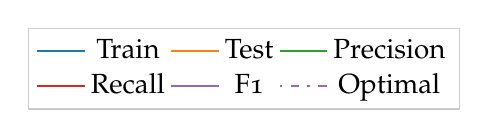
\begin{tikzpicture}

\definecolor{color0}{rgb}{0.12156862745098,0.466666666666667,0.705882352941177}
\definecolor{color1}{rgb}{1,0.498039215686275,0.0549019607843137}
\definecolor{color2}{rgb}{0.172549019607843,0.627450980392157,0.172549019607843}
\definecolor{color3}{rgb}{0.83921568627451,0.152941176470588,0.156862745098039}
\definecolor{color4}{rgb}{0.580392156862745,0.403921568627451,0.741176470588235}
\begin{axis}[%
 hide axis,
 xmin=10,
 xmax=50,
 ymin=0,
 ymax=0.4,
 legend columns=3,
 legend style={
   fill opacity=1,
   draw opacity=1,
   text opacity=1,
   align=center,
   anchor=north,
   draw=white!80!black
 },
 ]
 \addlegendimage{semithick, color0}
 \addlegendentry{Train};
 \addlegendimage{semithick, color1}
 \addlegendentry{Test};
 \addlegendimage{semithick, color2}
 \addlegendentry{Precision};
 \addlegendimage{semithick, color3}
 \addlegendentry{Recall};
 \addlegendimage{semithick, color4}
 \addlegendentry{F1};
 \addlegendimage{semithick, color4, dash pattern=on 1pt off 3pt on 3pt off 3pt}
 \addlegendentry{Optimal};
 \end{axis}

\end{tikzpicture}

  \end{subfigure}
  \par\bigskip
  \begin{subfigure}[b]{0.5\textwidth}
    \input{figures/optimizing-parameters/01-ferrenti-approach-176-LOG}
    \caption{}
    \label{fig:q1-LOG}
  \end{subfigure}%
    \hfill
  \begin{subfigure}[b]{0.5\textwidth}
    \input{figures/optimizing-parameters/01-ferrenti-approach-176-DT}
    \caption{}
    \label{fig:q1-DT}
  \end{subfigure}
  
  \begin{subfigure}[b]{0.5\textwidth}
    \input{figures/optimizing-parameters/01-ferrenti-approach-176-RF.tex}
    \caption{}
    \label{fig:q1-RF}
  \end{subfigure}%
   \hfill
  \begin{subfigure}[b]{0.5\textwidth}
    \input{figures/optimizing-parameters/01-ferrenti-approach-176-GB.tex}
    \caption{}
    \label{fig:q1-GB}
  \end{subfigure}
  \caption{{Four figures displaying hyperparameter search for the Ferrenti approach. The best estimator is visualized for all hyperparameters as a function of principal components during a grid search with a $5\times5$ stratified cross-validation, and the dotted lines mark the optimal hyperparameter-combination. Train stands for normal training accuracy, while test is the balanced accuracy on the test set. Precision, recall, and F1 scores are based on the test set. The number of principal components that explain the $95\%$ accumulated variance is $144$, while the optimal model is found using the F1-score.}}
  \label{fig:01-pca}
\end{figure}

\clearpage

\section*{Supplementary results}
Table~\ref{tab:03-probability-candidates} displays the 66 predicted candidates that all four machine learning models, using the data set derived in the intuitive approach, agreed on with a cut-off set to $0.75$. All band gaps are taken from the Materials Project database as calculated using DFT and the PBE functional. Note that materials can appear several times  on  the  list due  to  different  structures of the same composition. The  list  contains $5$ elementary (unary), $46$  binary and  $15$ ternary compounds. 

\begin{center}
\begin{longtable}{M{3.5cm} M{6.5cm} M{2.0cm}}
\caption{The $66$ predicted candidates that all models in the intuitive approach agreed on to a cut-off of $0.75$. All band gaps were taken from the Materials Project (MP) database, and materials can appear several times in the list due to different structures. The list contains $5$ elementary (unary), $46$ binary and $15$ ternary compounds.}
\label{tab:03-probability-candidates}  
\\ \hline
Compound formula & MP ID & Band gap from MP (eV) \\
\hline
  Ge & mp-137 & 0.87\\
  CdTe & mp-406 & 1.22\\
  HgSe & mp-820 & 0.12\\
  GeTe & mp-938 & 0.82\\
  MgTe & mp-1039 & 2.36\\
  CdSe & mp-1070 & 0.55\\
  GaSb & mp-1156 & 0.36\\
  BP & mp-1479 & 1.46\\
  MoSe$_2$ & mp-1634 & 1.41\\
  BN & mp-1639 & 4.64\\
  YbTe & mp-1779 & 1.52\\
  SnS & mp-1876 & 0.95\\
  SnTe & mp-1883 & 0.66\\
  GeTe & mp-2612 & 0.61\\
  AlSb & mp-2624 & 1.26\\
  CdSe & mp-2691 & 0.50\\
  SnSe & mp-2693 & 0.82\\
  CdSnAs$_2$ & mp-3829 & 0.30\\
  GaCuTe$_2$ & mp-3839 & 0.55\\
  ZnGeAs$_2$ & mp-4008 & 0.56\\
  ZnGeP$_2$ & mp-4524 & 1.20\\
  GaAgTe$_2$ & mp-4899 & 0.19\\
  CdSnP$_2$ & mp-5213 & 0.67\\
  GaCuS$_2$ & mp-5238 & 0.70\\
  SnS & mp-10013 & 0.23\\
  BAs & mp-10044 & 1.25\\
  GeSe & mp-10759 & 0.44\\
  MgSe & mp-10760 & 1.97\\
  CdTe & mp-12779 & 0.61\\
  MgSe & mp-13031 & 2.54\\
  MgTe & mp-13033 & 2.31\\
  TePb & mp-19717 & 1.05\\
  InAs & mp-20305 & 0.30\\
  InP & mp-20351 & 0.46\\
  InAgSe$_2$ & mp-20554 & 0.36\\
  InN & mp-22205 & 0.47\\
  AgI & mp-22894 & 1.39\\
  CuI & mp-22895 & 1.17\\
  CuBr & mp-22913 & 0.48\\
  CuCl & mp-22914 & 0.80\\
  AgI & mp-22919 & 1.00\\
  AgI & mp-22925 & 1.72\\
  Br & mp-23154 & 1.32\\
  TlI & mp-23197 & 2.25\\
  AgBr & mp-23231 & 0.79\\
  BC$_2$N & mp-30148 & 2.10\\
  CuI & mp-569346 & 1.21\\
  Hg & mp-569360 & 0.22\\
  Ga$_2$Os & mp-570875 & 0.66\\
  BC$_2$N & mp-629458 & 1.84\\
  InP & mp-966800 & 0.51\\
  GeC & mp-1002164 & 1.84\\
  TlP & mp-1007776 & 0.12\\
  BC$_2$N & mp-1008523 & 1.64\\
  BP & mp-1008559 & 1.07\\
  OsC & mp-1009540 & 0.17\\
  SiSn & mp-1009813 & 0.41\\
  ZnCdSe$_2$ & mp-1017534 & 1.85\\
  MgSe & mp-1018040 & 2.57\\
  AlSb & mp-1018100 & 0.91\\
  AlBi & mp-1018132 & 0.30\\
  Ge & mp-1067619 & 0.791\\
  Ga$_2$Ru & mp-1072429 & 0.12\\
  ZnCd$_3$Se$_4$ & mp-1078597 & 1.72\\
  BC$_2$N & mp-1079201 & 1.17\\
  Ge & mp-1198022 & 0.67\\
  \hline
\end{longtable}
\end{center}


Table~\ref{tab:04-probability-candidates} displays the $47$ predicted candidates that all four machine learning models and all three approaches agreed upon. The list contains $8$ elemental, $29$ binary, and $10$ tertiary compounds.

\begin{center}
\begin{longtable}{M{3.5cm} M{6.5cm} M{2.0cm}}
\caption{A table displaying the $46$? predicted candidates that all models and all approaches agree on.}
\label{tab:03-probability-candidates}  
\hline
Compound formula & MP ID & Band gap from MP (eV) \\
\hline
  P & mp-157 & 7.47\\
  SiRu & mp-189 & 0.63\\
  BN & mp-344 & 0.41\\
  HgSe & mp-820 & 3.96\\
  FeSi & mp-871 & 2.06\\
  MgTe & mp-1039 & 6.62\\
  CdSe & mp-1070 & 3.91\\
  BP & mp-1479 & 2.89\\
  CdSe & mp-2691 & 2.40\\
  ZnSiAs$_2$ & mp-3595 & 1.57\\
  ZnGeAs$_2$ & mp-4008 & 1.52\\
  CdSnP$_2$ & mp-5213 & 0.95\\
  Si$_2$Mo & mp-8938 & 0.66\\
  BAs & mp-10044 & 0.61\\
  GeSe & mp-10759 & 1.26\\
  N$_2$ & mp-12103 & 0.50\\
  BeSiN$_2$ & mp-15704 & 0.82\\
  InP & mp-20351 & 0.30\\
  InN & mp-22205 & 0.55\\
  AgCl & mp-22922 & 0.56\\
  I & mp-23153 & 1.20\\
  Br & mp-23154 & 0.19\\
  TlI & mp-23197 & 0.67\\
  AgBr & mp-23231 & 0.70\\
  H$_2$ & mp-23907 & 0.23\\
  Ge$_3$As$_4$ & mp-569600 & 1.25\\
  TlCl & mp-569639 & 0.44\\
  Sn$_3$As$_4$ & mp-570377 & 1.97\\
  H$_2$ & mp-634659 & 0.61\\
  N$_2$ & mp-672234 & 2.54\\
  TiFe$_2$Ge & mp-866375 & 2.31\\
  InP & mp-966800 & 1.05\\
  GeC & mp-1002164 & 0.30\\
  B$_2$AsP & mp-1008528 & 0.46\\
  BP & mp-1008559 & 0.36\\
  BeSiAs$_2$ & mp-1009087 & 0.47\\
  OsC & mp-1009540 & 1.39\\
  ScP & mp-1009746 & 1.17\\
  SiSn & mp-1009813 & 0.48\\
  SnC & mp-1009820 & 0.80\\
  AlBi & mp-1018132 & 1.00\\
  Al$_3$BN$_4$ & mp-1019380 & 1.72\\
  GeRu & mp-1025397 & 1.32\\
  PbS & mp-1057015 & 2.25\\
  Ge & mp-1067619 & 0.79\\
  ZnCd$_3$S$_4$ & mp-1078780 & 2.10\\
  Ga$_4$BiAs$_3$ & mp-1079228 & 1.21\\
  \hline
\end{longtable}
\end{center}



\bibliography{apssamp}% Produces the bibliography via BibTeX.

\end{document}

